\section{Реализация}
Решение приведенной выше задачи разрешения зависимостей является основной
функцией пакетного менеджера второго уровня. Выполнение этой функции обеспечивает
возможность установки пользователем любого пакета. Задача разрешения
зависимостей не имеет решения лишь в том случае, если присутствует
серьезное нарушение связи: для устновки пакету необходимо наличие
несущствующего пакета. Следствием такой ошибки является некорректная 
работа пакетного менеджера. Так как вся информация о пакетах и их 
зависимоятх отражается в индексе репозитория, обнаружить ошибку,
приводящую к столь серьезным последствиям, можно с помощью
контроля состояния индекса. Для этих целей в пакетном менеджере 
\textit{Deepsolver} реализованы утилиты для обновления индекса. 
Так как обеспечение целостности индекса - довольно трудная задача, а 
последствия ошибок очень серьезны, необходимо гарантировать своевременное
обнаружение недочетов в механизме обновления. Для этого осуществляется
проверка сформированного индекса, по результатам которой можно
судить о состоянии индекса, и, в случае возникновения ошибок, перейти
к более подробной диагностике непаладок в механизме обновления. 

Таким образом, можно сформилировать цели настоящей работы:
\begin{itemize}
\item{Создание утилиты для проверки готового индекса.}
\item{Тестирование утилит для обновления индекса.}
\end{itemize}

Помимо обнаружения критических ошибок, немаловажно отслеживать 
появление неактуальных данных, засчет которых неоправданно 
увеличивается размер индекса. Поэтому в цели работы входит
так же обнаружение подобного рода данных.

В качестве языка программирования для реализации решения был выбран \textit{Python (версия 2.7)}.

Основная функциональность решения представлена в модуле \textit{ds\_test.py}, который
будет подробно описан далее.

\subsection{Индекс репозитория Deepsolver}
Выше упоминалось , что вспомогательная информация о наборе пакетов репозитория
хранится в индексе. У \textit{Deepsolver} в каталоге \textit{base.*}, предназначенного для хранения индекса,
содержатся следующие файлы:\\
\begin{itemize}
\item{\textit{info} --- информационный файл с параметрами индекса;} 
\item{\textit{rpms.complete.data} --- вспомогательный файл, не предназначенный
для загрузки пользователями, с информацией для повторной фильтрации
provides;}
\item{\textit{rpms.data} --- основной список пакетов с информацией о зависимостях между ними;}
\item{\textit{rpms.descr.data} --- список пакетов с расширенными описаниями;}
\item{\textit{rpms.filelist.data} --- списки файлов для каждого бинарного пакета;}
\item{\textit{srpms.data} --- основная информация о пакетах с исходными текстами;}
\item{\textit{srpms.descr.data} --- список пакетов с исходными текстами, содержащий
расширенную информацию.}
\end{itemize} 
Каталог  \textit{base.*} существует для каждой архитектуры, \textit{i586}, \textit{x86\_64}, пакеты,
независящие от архитектуры, содержаться в каталоге \textit{noarch}.\\

\subsection{Использование Python для разработки консольных приложений}
\textbf{Python} --- высокоуровневый язык программирования общего назначения, ориентированный на повышение производительности разработчика и читаемости кода. Синтаксис ядра Python минималистичен. В то же время стандартная библиотека включает большой объём полезных функций\cite{wiki_python}.

Python поддерживает несколько парадигм программирования, в том числе структурное, объектно-ориентированное, 
функциональное, императивное и аспектно-ориентированное. Основные архитектурные черты --- динамическая типизация, 
автоматическое управление памятью, полная интроспекция, механизм обработки исключений, поддержка многопоточных вычислений 
и удобные высокоуровневые структуры данных. 
Код в Питоне организовывается в функции и классы, которые могут объединяться в модули (которые в свою очередь могут быть объединены в пакеты).

\subsubsection{Использование модуля argparse}
Начиная с версии \textit{Python 2.7}, в набор стандартных библиотек была включена 
библиотека \textit{argparse} для обработки аргументов (параметров, ключей) командной строки.

Эта библиотека использовалась при реализации приложений, описанных 
в разделах \ref{sn:index_test} и \ref{sn:patch_util_test}.

Кроме argparse в стандартной библиотеке \textit{Python} присутствуют еще два
решения для работы с аргументами командной строки: 
``getopt'' --- предоставляет интерфейс, аналогичный одноименной библиотеки для языка C,
и ``optparse'', являющийся по сути предшественником argparse.

Для обработки аргументов с помощью \textit{argparse} необходимо:
\begin{enumerate}
\item
Cоздать объект класса \textit{argparse.ArgumentParser()}.
\item
С помощью метода \textit{add\_argument()} добавить необходимые аргументы, причем они могут быть как
именованные, например ``-\ -path'', так и определяющиеся порядком их перечисления при вызове команды.

Кроме того для аргумента можно задать: значение по умолчанию, тип, к которому необходимо привести значение,
является ли он обязательным, строку-описание для вывода при запросе описания синтаксиса и т.п.

Например вызов

\textit{parser.add\_argument("square", type=int, help="display a square of a given number")}

определяет первым аргументов приложения ``square'' целочисленного типа с описанием.
\item
После этого необходимо вызвать метод \textit{parse\_args} у объекта парсера,
передав в качестве аргумента список ``sys.argv''.
\item
В случае корректного указания аргументов при вызове приложения
этот метод вернет объект-словарь, поля которого содержат значения одноименных
аргументов, причем их типы соответсвуют указанным при вызове \textit{add\_argument()}
или содержат значения по умолчанию.
\item
В случае, если пользователь некорректно указал аргументы, либо запустил приложение
с ключом \textit{-h}, пользователю будет выведено автоматически сгенерированное сообщение
вида:

\textit{\$ prog.py -h
usage: prog.py [-h] [--sum] N [N ...]\\
Process some integers.\\
positional arguments:
 N           an integer for the accumulator\\
optional arguments:
 -h, --help  show this help message and exit
 --sum       sum the integers (default: find the max)
}
\end{enumerate}

Кроме того \textit{argparse} поддерживает формирование в рамках одного приложения
подпрограмм с совершенно различной семантикой таким образом, что
для каждой из них может быть создан свой объект-парсер аргументов,
который следует добавить в корневой парсер с помощью метода \textit{add\_subparsers()}.

\subsubsection{Использование объектов-генераторов}
\label{ssn:generators}
В языке \textit{Python} на синтаксическом уровне поддерживаются итераторы\cite{gamma} ---
типовое решения для инкапсуляции последовательного доступа к элементам объекта-агрегата.

Языковые конструкции \textit{for, map, reduce, filter} и т.д. принимают в качестве аргументов
итерируемые объекты, например списки, множества.

Кроме этих стандартных реализаций разработчик может добавить свои реализации итераторов,
для этого необходимо определить классы с методами \textit{\_\_iter\_\_()} и \textit{next()}.
Причем первый должен вернуть итерируемые объект, а второй --- следующий элемент итерации, либо 
вызвать исключение \textit{StopIteration}, если итерация логически завершилась.

Одной из интересных возможностей языка являются генераторы --- функции, 
сохраняющие внутреннее состояние: значения локальных переменных и текущую инструкцию. 
Генераторы могут использоваться как итераторы для структур данных и для ленивых вычислений.

При вызове генератора функция немедленно возвращает объект-итератор, 
который хранит текущую точку исполнения и состояние локальных переменных функции. 
При запросе следующего значения (посредством метода next(), неявно вызываемого в for цикле) 
генератор продолжает исполнение функции от предыдущей точки останова до следующего оператора yield или return.

\begin{lstlisting}[frame=single]
def fibonacci(max):        
    a, b = 0, 1
    while a < max:
        yield a            
        a, b = b, a + b    

for n in fibonacci(100):   
    print n,               

\end{lstlisting}

Выше приведен пример использования генераторов для вычисления чисел Фибоначчи.
Функция \textit{fibonacci()} содержит в себе оператор \textit{yield}, поэтому при ее вызове
возвращается не целое число --- последнее из чисел Фибоначчи, а генерератор.

В цикле for неявно вызываются методы генерератора \textit{\_\_iter\_\_()} и \textit{next()},
причем для каждого вызова \textit{next()} происходит исполнение функции до остановки после 
оператора \textit{yield a}, либо выход из функции, в этом случае генератор 
вызывает исключение исключение \textit{StopIteration}.

В Python 2.4 появились генераторные выражения — выражения, дающие в результате генератор. 
Генераторные выражения позволяют сэкономить память там, где иначе требовалось бы использовать список с промежуточными результатами:

\textit{ >>> sum(i for i in xrange(1, 100) if i \% 2 != 0)}

В этом примере суммируются все нечётные числа от 1 до 99.

Начиная с версии 2.5, Python поддерживает полноценные сопроцедуры: теперь в генератор можно передавать значения 
с помощью метода \textit{send()} и возбуждать в его контексте исключения с помощью метода \textit{throw()}.

\subsection{Модуль ds\_test.py}
\textit{ds\_test.py} предоставляет основную функциональность утилиты  как для тестирования
готового индекса, так и для проверки после обновления. Ниже представлена диаграмма~классов данного модуля.\\
%%FIXME:Диаграмма классов
\\
\begin{figure}[!ht]
\begin{center}
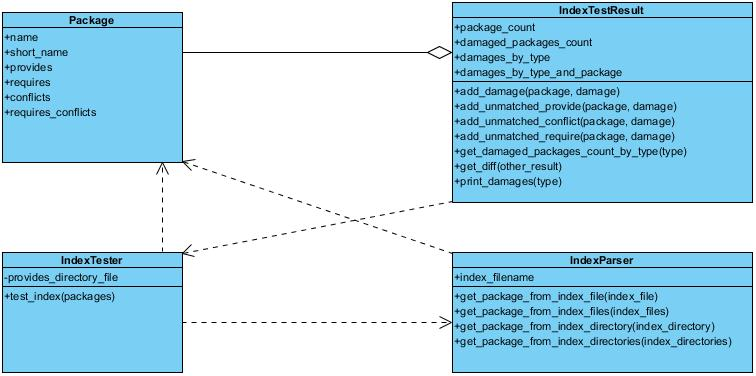
\includegraphics[scale=0.6, clip]{../resources/uml/ds_test_class_diagram.jpg}
\caption{Диаграмма классов модуля ds\_test.py}
\label{gr:dstestclassdiag}
\end{center}
\end{figure}

\textit{Package} - это класс, объекты которого представляют отдельные пакеты и, как видно из диаграммы,
содержат информацию о пакете, получаемую из входного файла: поля строкового типа \textit{name} и 
\textit{short\_name}, а так же массивы строк \textit{provides}, \textit{requires}
и \textit{conflicts}, соответствующие одноименных множествам зависимостей пакета.
\\

Класс \textit{IndexParser} отвечает за разбор файлов индекса, в качестве параметра конструктора
ожидается файл, который необходимо обработать. Метод \textit{\_append\_index\_filename} получает на вход
имя директории с целевым файлом и образует из него и имени файла для парсинга
путь.

Основным методом класса \textit{IndexParser} является \textit{get\_packages\_from\_index\_file}.
В качестве входных данных используется сформированный ранее путь к файлу с данными
для парсинга. 

Этот метод возвращает генератор (см. \ref{ssn:generators}) массива объектов класса \textit{Package},
передавая в конструкторе значения полей класса, полученных в результате разбора.\\

Тот факт, что метод \textit{get\_packages\_from\_index\_file} возвращает генератор позволяет
его использовать в том числе и для парсинга большого количества файлов большого размера, 
таким образом, что все множество пакетов необязательно должно сохраняться в память ---
при каждой новой итерации будет прочитан следующий один блок файла индекса, 
а содержание предыдущего может быть удалено из ОЗУ.

При этом пользователи класса могут работать с полученным генератором, как с обычным списком пакетов.

Так как каждый из файлов индекса храниться в виде архива в формате \textit{GNU Zip}, 
необходимо было решить проблему чтения архивированных файлов.

В итоговой реализации было принято решение использовать модуль \textit{gzip}, 
входящий в набор стандартных библиотек Python, и реализующий интерфейс доступа к файлам,
аналогичный тому, которй предоставляется при чтении обычных файлов.

Класс \textit{IndexTestResult} предназначен для удобной работы с результатами тестирования. 
У этого класса есть три метода отвечающие за накопление результатов тестирования:
\textit{add\_unmatched\_provide}, \textit{add\_unmatched\_require} и \textit{add\_unmatched\_conflict}, каждый из которых
в качестве первого аргумента получает объект класса \textit{Package} - текущий пакет, а в качестве второго
- строку, соответствующую повреждению(из списка \textit{provides}, \textit{requires} или \textit{conflicts}).

Для управления выводом переопределен метод \textit{\_\_str\_\_}. Так же у класса существует метод \textit{diff},
принимающий в качестве аргумента объект класса \textit{IndexTestResult}. У объекта, 
вызывающего этот метод, изменяется список повреждений в соответствии с содержимым обхекта,
переданного в аргументах: в результате, основной объект содержит только новые повреждения,
то ест отсутствующие в объекте-аргументе.\\

В классе \textit{IndexTester} определены методы, непосредственно отвечающие за тестирование
индекса. При создании объекта данного класса в конструкторе передается файл с директориями,
в которых может находится \textit{provide}, не считаясь избыточным. 
Алгоритм тестирования реализован в методе \textit{test\_index}. Этот метод на вход
получает массив объектов класса \textit{Package}. Алгоритм выглядит следующим образом:
\begin{enumerate}
\item{Инициализация списка имен пакетов - \textit{names\_set}, списка \textit{provides} и 
списка \textit{requires\_conflicts}}
\item{Совершается проход в цикле по всем пакетам. На каждом шаге 
к уже сформированным спискам \textit{provides}, \textit{requires\_conflicts} и \textit{names\_set} 
добавляются данные текущего пакета. В результате получаем набор списков \textit{provides}, 
\textit{requires\_conflict} и имен для набора пакетов}
\item{Создается объект класса \textit{IndexTestResult}}
\item{Совершается проход в цикле по всем пакетам. На каждом шаге цикла проверяется}
\end{enumerate}
\begin{itemize}
	\item{Для каждого \textit{provide} пакета проверяется является ли он избыточным: существует ли
	строка из списка \textit{requires\_conflicts} или находится ли он в одной из заданных директорий.
	Если не является, то данный пакет помечается, как поврежденный, а данный provide помечается,
	как избыточный, то есть вызывается метод \emph{add\_unmatched\_provide} у объекта класса \textit{IndexTestResult}}
	\item{Для каждого \textit{require} пакета проверяется не является ли он анметом: существует ли
	соответствующая строка из списка \textit{provides}. Если не существует, то пакет помечается, как 
	поврежденный, а \textit{require}, как \textit{анмет}, то есть вызывается метод \textit{add\_unmatched\_require}
	у объекта класса \textit{IndexTestResult}}
	\item{Для каждого \textit{conflict} пакета проверяется не является ли он избыточным: существует ли
	соответствующая строка из списка \textit{provides}. Если не существует, то пакет помечается, как 
	поврежденный, а \textit{conflict}, как поврежденный, то есть вызывается метод \textit{add\_unmatched\_conflict}
	у объекта класса \textit{IndexTestResult}}
	\item{Возвращается объект класса \textit{IndexTestResult}}
\end{itemize}

\subsection{Утилита для проверки готового индекса}
\label{sn:index_test}
\subsubsection{Формат входных данных}
Для тестирования целостности репозитория используются данные из файла \textit{rpms.data},
в котором описание каждого пакета соответствует следующему формату:
\begin{itemize}
\item{[name-version-release.architecture.rpm] }
\item{n=name} 
\item{e=epoch}
\item{v=version}
\item{r=release}
\item{arch=architecture}
\item{btime=build time}
\item{p:provide}
\item{r:require}
\item{c:conflict}
\item{o:obsolete}
\end{itemize}
Очевидно, что каждому пакету соответствует набор множеств \textit{provides},
\textit{requires}, \textit{conflicts}, \textit{obsoletes}, которые могут быть и пустыми.\\

Под целостностью репозитория понимается состояние, которое удовлетворяет следующим
условиям:
\begin{itemize}
\item{Для каждого \textit{require} пакета существует одноименный \textit{provide} 
другого пакета. Require, для которого это условие не выполняется
называется \textit{анметом (unmet)}. }
\item{Для каждого \textit{provide} существует одноименный \textit{require/conflict} или
он находится в директории из заранее заданного списка.Это условие 
контролирует появление избыточных \textit{provide}, засчет которых %%FIXME:сделать ссылку на место, где про это говорилось
может существенно расти размер индекса.}
\item{Для каждого \textit{conflict} пакета существует одноименный \textit{provide} 
другого пакета. Это условие не является таким строгим, как два предыдущих,
но желательно, чтобы оно выполнялось. }
\end{itemize}

В качестве входных данных используется файл с содержимым формата, описанного выше,
и расширением \textit{*.data.gz}.

\subsubsection{Детали реализации}
\begin{figure}[!ht]
\begin{center}
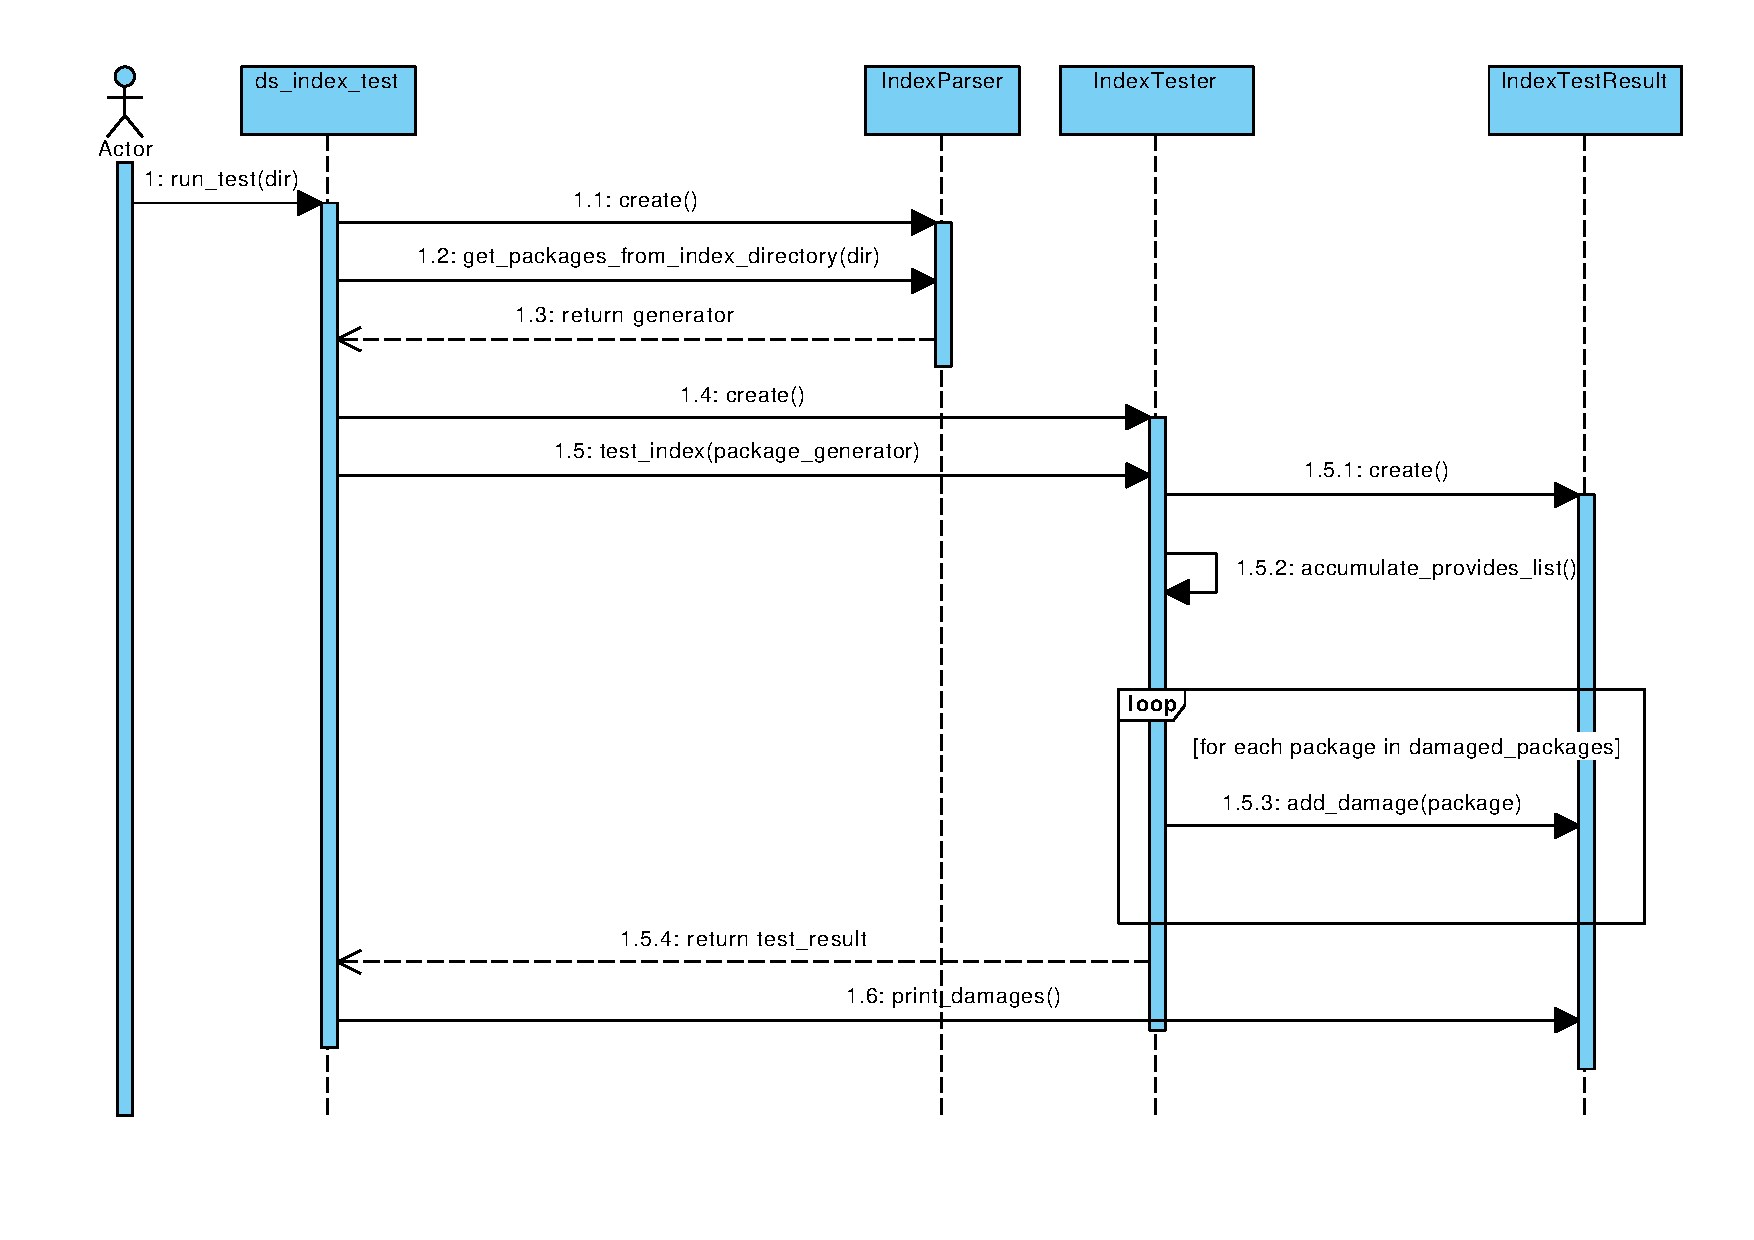
\includegraphics[scale=0.6, clip]{../resources/uml/SimpleTestCase.pdf}
\caption{Диаграмма последовательности алгоритма проверки индекса}
\label{gr:simple_test_case}
\end{center}
\end{figure}

Таким образом, первый этап проверки сводится к выполнению следующих действий (см. \ref{gr:simple_test_case}):

\begin{enumerate}
\item
После запуска утилиты создается объект класса \textit{IndexParser} и вызывается его метод
\textit{get\_packages\_from\_index\_directory()}, куда в качестве выбранной
директории передается строка, полученная в качестве аргумента утилиты.

\item
В качестве результата работы метод \textit{get\_packages\_from\_index\_directory()}
возвращается объект-генератор, элементами которого являются отдельные пакеты из индекса 
репозитория.

\item
После этого создается объект класса \textit{IndexTester} и вызывается его метод
\textit{test\_index()} для объекта-генератора, полученного на предыдущем шаге.

\item
Перед началом работы метода \textit{test\_index()} происходит сбор всех существующих
в индексе версий пакетов и их provides-строк. Полученное множество строк сохраняется
в виде хэш-таблицы для обеспечения оптимального времени поиска.

\item
Таким образом для определения наличия повреждений целостности
необходимо проверить, что для каждого из requires и provides всех пакетов
существует соответсвующее вхождение в хэш-таблице из предыдущего шага.

\item 
Для каждого найденного повреждения необходимо добавить его в объект \textit{IndexTestResult}.

\item
После чего пользователю выводится подробная статистическая информация о найденных повреждениях.

\end{enumerate}

\subsubsection{Формат выходных данных}

На выходе получается статистика вида:\\
\\
Found [количество найденных пакетов] packages\\
.[количество поврежденных пакетов] packages are damaged\\
.[количество пакетов с избыточными provide] packages have unmatched provides\\
.[количество пакетов с анметами] packages have unmets\\
.[количество пакетов с избыточными conflict] packages have unmatched conflicts\\

Подробная информация о повреждениях регулируется с помощью ключей и имеет следующий формат:\\
package [имя пакета] has unmatched [тип: provide или conflict] [строка соответствующая повреждению]\\
package [имя пакета] has [тип: unmet] [строка соответствующая повреждению]\\

\subsection{Проверка утилит для обновления индекса}
\label{sn:patch_util_test}
Для данной проверки в качестве входных данных необходимо предоставить
путь до каталога \textit{base.*}, так как утилиты \textit{ds-patch} и 
\textit{ds-provides} используют данные всех файлов из директории.

Под утилитами для обновления индекса подразумеваются описанные
выше \textit{ds-patch} и \textit{ds-provides}.

Проверка представляет собой последовательность действий:

\begin{itemize}
\item{Проведение начального тестирования на неизменном индексе. Сохранение
и вывод результатов.}
\item{Совершаем проход в цикле по каждой директории из \emph{INDEX\_FILES\_PATH}. На
каждом шаге:
	\begin{itemize}
	\item{Формируем список пакетов для текущей директории.}
	\item{Для каждого пакета из списка вызывается утилита \textit{ds-patch }
	для текущего пакета, затем \textit{ds-provides} для директории файла, а 
	так же связанных с ней. После этого проводится тестирование
	измененного индекса и вывод результатов отличных от начальных
	с использование метода \textit{diff} объекта класса \textit{IndexTestResult}.}
	\end{itemize}
}
\end{itemize}

В качестве результата данная утилита предоставляет статистику выше описанного формата,
полученную сначала на готовом индексе, а затем после каждого запуска утилит для обновления
индекса. Отображение выходных данных этой утилиты так же регулируется ключами.

\subsection{Результаты}
Тестирование проводилось на реальных данных репозитория \textit{Deepsolver}.
Начальный этап проверки, направленный на выявление ошибок в уже сформированном репозитории,
проводился для индекса до официального внедрения индекса \textit{Deepsolver}, так и 
после.\\

\paragraph{Тестирования индекса до официального внедрения Deepsolver\\}
На этом этапе на основании индексов всех архитектур (\textit{i586, x86\_64, noarch})
насчитывалось 65 345 пакетов.

Для пары индексов  \textit{x86\_64, noarch} было обнаружено 4 избыточных \textit{provides}, 
обнаруженных у одного пакета из \textit{noarch}, что тем не является идентефикатором серьезной
ошибки, имеющей деструктивные последствия, так как у \textit{noarch} - особый статус: он должен
содержать \textit{provides}, удовлетворяющие как \textit{x86\_64}, так и \textit{i586}. Побочным
эффектом этого требования является появление такого рода избыточных provides.

Для пары индексов \textit{i586, noarch} критических ошибок обнаружено не было.

При проверки индексов для всех архитектур было обнаружено 831 избыточных conflicts, что
критической ошибкой не является.

\paragraph{Тестирование индекса после официального внедрения\\}
На данном этапе для всех архитектур было обнаружено 55 346 пакетов, никаких
ошибок выявлено не было.\\

\paragraph{Тестирование утилит для обновления индекса}
При проверке механизма удаления пакетов после каждого  запуска утилит, то есть
после каждого удаления и перефильтрации \textit{provides}, иногда обнаруживались
анметы, которые являлись следствием зависимостей на сами удалённые пакеты. Так 
как репозиторий - это нечто целостное, и он содержит множество разнообразных пакетов
с колоссальным количеством взаимосвязей между ними, то удаление пакета
естественно будет приводить к нарушению каких-то связей. Поэтому обнаруженные ошибки
опять же не являются свидетельством некорректной работы утилит.













